\section{Case Study: Key-Value Store}
\label{sec:kvs}
The next two sections contain case studies that show how \lang can be used to
build practical distributed programs. Both case studies are monotonic programs:
that is, both programs consist of monotone functions applied to lattices. This
ensures that the values computed by the programs ``grow'' over time---these
examples show the various kinds of forward progress that can be encoded using
\lang.

In the first case study, we show that a distributed key-value store can be
\emph{composed} via a series of monotone mappings between simple lattices. This
demonstrates that \lang's built-in lattices are useful and results in a very
concise implementation. Moreover, it gives us confidence in the correctness of
our implementation, because much of the program's complexity is handled by the
behavior of the built-in lattices, which are likely to be correct.
\paa{not sure what to suggest, but this last clause seems underconfident 
(and slightly run-on).
perhaps we just want to say that we assert them to be correct, or that it's easy
to prove/convince ourselves that they are correct due to their simplicity, etc}

\subsection{Basic Architecture}
\begin{figure}[t]
\begin{scriptsize}
\begin{lstlisting}
module KvsProtocol
  state do
    channel :kvput, [:reqid, :@addr] => [:key, :val,
                                         :client_addr]
    channel :kvput_resp, [:reqid] => [:@addr, :replica_addr]
    channel :kvget, [:reqid, :@addr] => [:key, :client_addr]
    channel :kvget_resp, [:reqid] => [:@addr, :val,
                                      :replica_addr]
  end
end
\end{lstlisting}
\end{scriptsize}
\caption{Key-value store interface.}
\label{fig:kvs-interface}
\end{figure}

\begin{figure}[t]
\begin{scriptsize}
\begin{lstlisting}
class KvsReplica
  include Bud
  include KvsProtocol

  state { lmap :kv_store } (*\label{line:kvs-map-ddl}*)

  bloom do
    kv_store   <= kvput {|c| {c.key => c.val}} (*\label{line:kvs-put-merge}*)
    kvput_resp <~ kvput {|c| [c.reqid, c.client_addr, ip_port]}
    kvget_resp <~ kvget {|c| [c.reqid, c.client_addr,
                              kv_store.at(c.key), ip_port]}
  end
end
\end{lstlisting}
\end{scriptsize}
\caption{KVS replica implementation in \lang.}
\label{fig:kvs-replica}
\end{figure}

Key-value stores (KVS) such as Chord~\cite{Stoica2001} and
Dynamo~\cite{DeCandia2007} are a popular choice for distributed storage. A KVS
provides a lookup service that allows client applications to retrieve the
\emph{value} associated with a given \emph{key}. In a typical KVS, key-value
pairs are replicated on multiple server replicas for redundancy and the keyspace
is partitioned in some fashion to improve aggregate storage and
throughput. \emph{Eventual consistency} is a common correctness criteria: after
all client updates have reached all storage nodes, all the replicas of a
key-value pair will converge to the same final state~\cite{Terry1995,vogels}.

Figure~\ref{fig:kvs-interface} shows a simple KVS interface in \lang. Client
applications submit \emph{get(key)} and \emph{put(key, val)} operations by
inserting into the \texttt{kvget} and \texttt{kvput} channels, respectively;
server replicas return responses via the \texttt{kvget\_resp} and
\texttt{kvput\_resp} channels.
\paa{what is kvput\_response for?  will I learn in section 5.2?}

Figure~\ref{fig:kvs-replica} contains the \lang code for a KVS server
replica. An \texttt{lmap} lattice is used to maintain the mapping between keys
and values (line~\ref{line:kvs-map-ddl}). Since the values in an \texttt{lmap}
lattice must themselves be lattice elements, for now we assume that clients only
want to store and retrieve lattice values; we discuss how to support arbitrary
values in Section~\ref{sec:kvs-versions}. To handle a \emph{put(key, val)}
request, a new \emph{key} $\to$ \emph{val} map is created and merged into
\texttt{kv\_store} (line~\ref{line:kvs-put-merge}). If \texttt{kv\_store}
already contains a value for the given key, the two values will be merged
together using the value lattice's merge function (see
Section~\ref{sec:lattice-built-ins} for details). Note that we use the \lang
features described in Section~\ref{sec:bloom-interop} to enable interoperability
between code that accesses traditional Bloom collections (e.g., channels) and
lattices (e.g., the \texttt{kv\_store} lattice).  Note that \texttt{ip\_port} is
a built-in function that returns the IP address and port number of the current
Bud instance.

The state of two replicas can be synchronized by simply exchanging their
\texttt{kv\_store} maps; the \texttt{lmap} merge function will automatically
resolve all conflicting updates made to the same key. This property allows
considerable flexibility in how replicas can choose to propagate updates.
% TODO: (1) finish repl discussion (composition, replication strat) (2) partitioning

\subsection{Object Versioning}
\label{sec:kvs-versions}

The initial KVS design is sufficient for applications that want to store
monotonically increasing values, such as session logs or increasing counters. To
allow arbitrary updates to be made to the stored values, we now consider how to
support \emph{object versions}. This is a classic technique for recognizing
mutual inconsistency between members of a distributed system~\cite{Parker1983};
our design is similar to that used by Dynamo~\cite{DeCandia2007}.

Each replica associates keys with
$\langle\textit{vector-clock},\textit{value}\rangle$ pairs. The vector clock
(VC) captures the causal relationship between different versions of a
record~\cite{Fidge1988,DeCandia2007}. Clients get and put
$\langle\textit{vector-clock},\textit{value}\rangle$ pairs. When a client
updates a value it has previously read, the client increments its own position
in the VC and includes the updated vector clock $V_U$ with its \emph{put}
operation. Upon receiving an update, the server compares $V_U$ with the VC of
the server's version of the record ($V_S$). If $V_U > V_S$, the server replaces
the stored record with the client's update. If $V_S > V_U$, the update is
ignored (this situation might arise due to duplication and reordering of
messages by the network). If $V_U$ and $V_S$ are incomparable, the two versions
of the record are concurrent, so a client-supplied reconciliation function is
used to resolve the conflict.

From a \lang perspective, each replica still stores a monotically increasing
value---the only difference is that in this scheme, the \emph{version} stored by
a replica increases over time, rather than the associated value. Hence, we now
consider how to support vector clocks and version-value pairs using \lang.

\subsubsection{Vector Clocks}
\nrc{Ugh, TODO.}
Vector clocks are a well-known mechanism for recording the causal relationships
between events~\cite{Fidge1988}. A vector clock is a map from node identifiers
to logical clocks. Each event $e$ is associated with a vector clock $V_e$; if
$V_e < V_{e'}$, $e$ causally precedes $e'$.

In \lang, vector clocks can be represented as an \texttt{lmap} that maps node
identifiers to \texttt{lmax} values. This seems reasonable, since logical clock
values (\texttt{lmax}) can only increase over time. The merge function provided
by \texttt{lmap} achieves the desired semantics.

\subsubsection{Version-Value Pairs}
\begin{figure}[t]
\centering
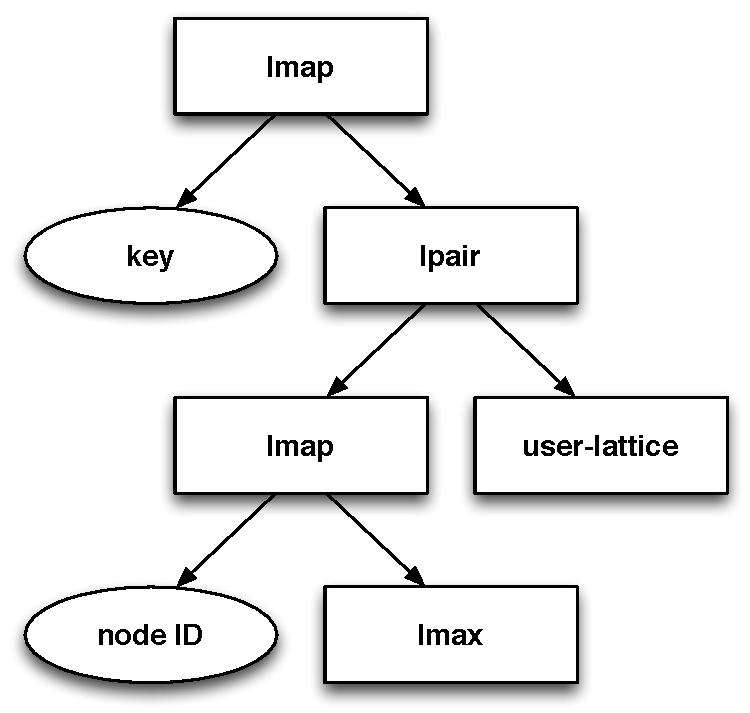
\includegraphics[width=0.8\linewidth]{fig/kvs-vc-lattice.pdf}
\caption{Nested lattices in a KVS with object versioning.}
\label{fig:kvs-vc-lattices}
\end{figure}


\subsection{Quorum Replication}
